% !TEX root = ../main.tex
% SECTION 5: MAGNETFELD
% ============================================================

\StartChapter{Magnetfeld}

\begin{runintext}
Grundlagen des \ZSFkeyword*{Magnetfelds}: magnetische Kräfte auf bewegte Ladungen und Ströme, die Erzeugung von \ZSFkeyword*{B-Feldern} durch Leiter (\ZSFkeyword*{Biot-Savart}, \ZSFkeyword*{Ampère}) sowie magnetische Eigenschaften der Materie. Zentral für Aufgaben zur Teilchenablenkung und Felderzeugung.
\end{runintext}
\begin{runintext}
\ZSFkeyword*{Feldlinien} bilden immer geschlossene Schleifen (keine magnetischen Monopole).
\end{runintext}

\SubsectionBar[sec:lorentz-force]{Lorentz}
\ZSFindex{Magnetfeld}
\ZSFindex{B-Feld}
\ZSFindex{Magnetische Flussdichte}
\ZSFindexsee{Tesla}{Magnetische Flussdichte}
\ZSFindex{Kraft / Kraft auf Leiter}
\begin{runintext}
Die elementare \ZSFkeyword[Lorentzkraft]{Kraft} auf Einzelteilchen und Leiterstücke im externen Magnetfeld; wichtig für prinzipielle Krafteinwirkungen.
\end{runintext}

\ZSFfig{graphics/Elektromagnetismus_Rechte_Hand_Regel_Lorentzkraft_Vektoren.png}{Rechte-Hand-Regel}{Daumen $\vec{v}$, Zeige $\vec{B}$, Mittel $\vec{F}$ (für $+q$)}

\begin{formulabox}[Lorentzkraft auf Punktladung]
\[ \vec{F} = q\,\vec{v}\times\vec{B} \quad \text{bewegte Ladung} \]
\[ 1\,\si{T} = 1\,\si{N}/(\si{A}\cdot\si{m}) \quad 1\,\si{G} = 10^{-4}\,\si{T} \]
\formulanote{Kraft $\vec{F} \perp \vec{v}$ und $\vec{F} \perp \vec{B}$. Für negative Ladungen ($q<0$) kehrt sich die Kraftrichtung um (Erdmagnetfeld $\approx 0.5\,\si{G}$).}
\end{formulabox}

\begin{formulabox}[Kraft auf strombeflossene Leiter]
\[ \mathrm{d}\vec{F} = I\,\mathrm{d}\vec{\ell}\times\vec{B} \quad \text{Stromelement (differentiell)} \]
\[ \vec{F} = I\,\vec{\ell}\times\vec{B} \quad \text{gerader Leiter (homogenes Feld)} \]
\formulanote{Vektor $\vec{\ell}$ zeigt in Stromrichtung $I$ mit Leiterlänge $\ell = |\vec{\ell}|$.}
\end{formulabox}

\begin{formulabox}[Kraft zwischen parallelen Leitern]
\[ \frac{F}{\ell} = \frac{\mu_0\,I_1\,I_2}{2\pi\,r} \quad \text{parallele Leiter} \]
\formulanote{Kraft pro Länge im Abstand $r$ ($\ell$: Länge des betrachteten Leiterabschnitts). Gleichsinnig anziehend, gegensinnig abstossend.}
\end{formulabox}

\begin{defbox}[Kraft auf Leiter im Magnetfeld]
\begin{splitbox}[0.48]
    \centering
    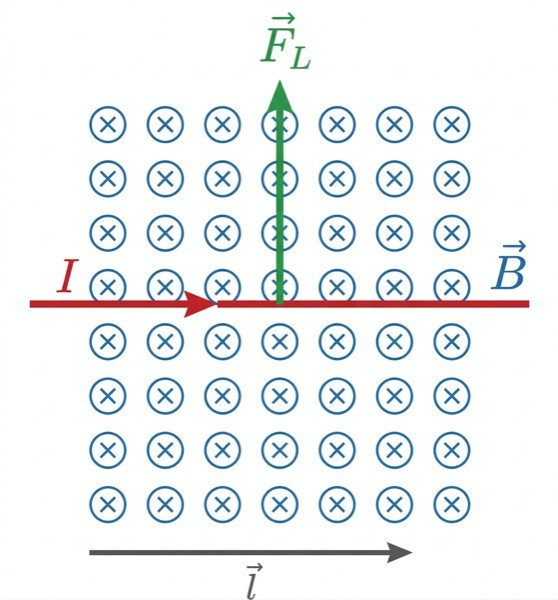
\includegraphics[width=\linewidth, keepaspectratio]{graphics/Lorentzkraft_gerader_Leiter_im_Magnetfeld.jpg}
    \ZSFfigcaption{Gerader Leiter: Kraft $\vec{F}=I\,\vec{\ell}\times\vec{B}$}
    \tcblower
    \centering
    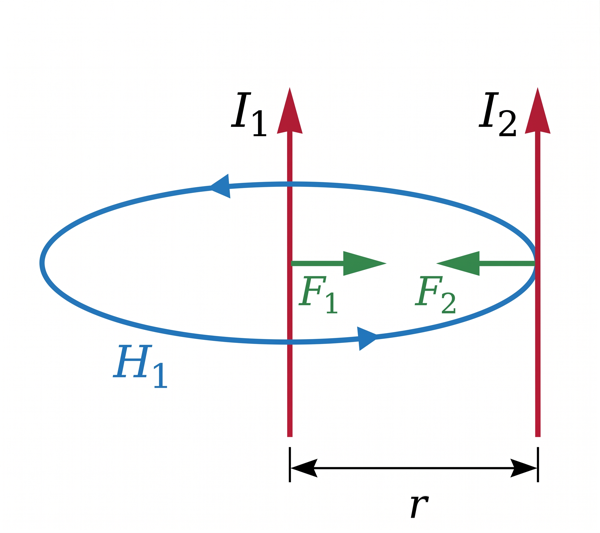
\includegraphics[width=\linewidth, keepaspectratio]{graphics/Elektrodynamik_Parallele_Leiter_Lorentzkraft_Anziehung.png}
    \ZSFfigcaption{Parallele Leiter: Gleichsinnig $\to$ anziehend, gegensinnig $\to$ abstossend}
\end{splitbox}
\end{defbox}

\SubsectionBar[sec:particle-in-bfield]{Teilchen im B-Feld}
\ZSFindex{Wien-Filter}
\ZSFindexsee{Geschwindigkeitsfilter}{Wien-Filter}
\ZSFindex{Zentripetalkraft}
\ZSFindex{Zyklotronfrequenz/-periode}
\ZSFindex{Beschleunigung}
\begin{runintext}
Dynamik von geladenen Teilchen in Magnetfeldern, speziell \ZSFkeyword[Kreisbahn]{Kreisbahnen} und \ZSFkeyword[Massenspektrometer]{Massenspektrometrie}.
\end{runintext}
\begin{runintext}
Senkrecht zu $\vec{B}$: \ZSFkeyword{Kreisbahn}; Periode/Frequenz unabhängig von $r$ und $v$.
\end{runintext}
\begin{formulabox}
\[ |q|\,v\,B = m\,\frac{v^2}{r} \implies r = \frac{m\,v}{|q|\,B} = \frac{p}{|q|\,B} = \frac{\sqrt{2m E_{\mathrm{kin}}}}{|q|\,B} \]
\formulanote{Kreisbahn: Lorentzkraft = Zentripetalkraft; Bahnradius $r$ über $v$, Impuls $p$ oder kin.\ Energie $E_{\mathrm{kin}}$.}
\end{formulabox}

\begin{formulabox}
\[ T = \frac{2\pi m}{|q|B} = \frac{2\pi r}{v} \quad \text{Zyklotronperiode} \]
\[ f = \frac{1}{T} = \frac{|q|B}{2\pi m} \quad \text{Zyklotronfrequenz} \]
\[ \omega = 2\pi\,f = \frac{|q|\,B}{m} \quad \text{Zyklotron-Winkelfrequenz} \]
\formulanote{Umlaufzeit $T$, Frequenz $f$ und $\omega$ hängen nur von $q/m$ und $B$ ab (unabhängig von $r$ und $v$!).}
\end{formulabox}

\begin{formulabox}
\[ |\vec{v}| = \frac{|\vec{E}|}{|\vec{B}|} \quad \text{Geschwindigkeitsfilter (Wien-Filter)} \]
\formulanote{Wien-Filter: $\vec{E}\perp\vec{B}$. Die Kräfte $F_{\mathrm{el}}=qE$ und $F_{\mathrm{Lorentz}}=qvB$ heben sich auf für $v=E/B$ (Teilchen fliegen geradeaus).}
\end{formulabox}

\begin{formulabox}
\[ q\,U = \frac{1}{2}\,m\,v^2 \implies \frac{m}{|q|} = \frac{B^2\,r^2}{2\,U} \]
\formulanote{Massenspektrometer: Beschleunigung mit Spannung $U$, anschliessend Ablenkung auf Radius $r$ im homogenen Feld $B$.}
\end{formulabox}
\begin{runintext}
\ZSFkeyword*{Thomson}: $q/m$ über gekreuzte Felder + E-Ablenkung. \ZSFkeyword{Massenspektrometer}: $q/m$ aus Bahnradius.
\end{runintext}


\ZSFmanualColumnBreak
\SubsectionBar[sec:magnetic-moment-torque]{Moment, Drehmoment}
\ZSFindex{Drehmoment}
\ZSFindex{Kraft / Kraft auf Leiter}
\ZSFindex{Magnetisches Moment}
\begin{runintext}
Wirkung von Magnetfeldern auf \ZSFkeyword[Stromschleife]{Stromschleifen} (\ZSFkeyword[Magnetischer Dipol]{magnetische Dipole}); relevant z.\,B. für Elektromotoren.
\end{runintext}

\begin{figbox}[Drehmoment Leiterschleife]
\centering
\begin{tikzpicture}[scale=1.45, >={Stealth[length=1.6mm]}, line cap=round]
  \fill[gray!10] (0.80,0.55) ellipse (0.72 and 0.24);
  \draw[line width=0.8pt] (0.80,0.55) ellipse (0.72 and 0.24);
  \node[inner sep=0.2mm] at (0.46,0.68) {\tiny $A$};
  \draw[->, red!60!black, line width=0.9pt] ([shift={(-70:0.72 and 0.24)}]0.80,0.55) arc[start angle=-70, end angle=-38, x radius=0.72, y radius=0.24];
  \node[red!60!black, inner sep=0.2mm] at (1.46,0.20) {\tiny $I$};
  \draw[->, line width=0.4pt] (0.80,0.55) -- ([shift={(-15:0.72 and 0.24)}]0.80,0.55);
  \node[inner sep=0.2mm] at (1.12,0.66) {\tiny $R$};
  \draw[->, thick, \chaptercolor] (0.80,0.62) -- (0.80,1.78);
  \node[\chaptercolor, inner sep=0.2mm] at (0.97,1.70) {\tiny $\vec{\mu}$};
  \node[inner sep=0pt] at (0.80, -0.05) {\tiny (a) Dipolmoment $\vec{\mu} = I\vec{A}$};
\end{tikzpicture}%
\quad
\begin{tikzpicture}[scale=1.45, >={Stealth[length=1.6mm]}, line cap=round]
  \foreach \fy in {0.55, 1.05, 1.55} {%
    \draw[->, gray!40, line width=0.4pt] (0.05,\fy) -- (1.52,\fy);
    \draw[->, gray!40, line width=0.4pt] (0.05,\fy) -- (0.80,\fy);}
  \node[gray!70!black, inner sep=0.2mm] at (1.42,1.66) {\tiny $\vec{B}$};
  \fill[\chaptercolor!8] (0.83,1.05) -- (1.09,1.05) arc[start angle=0, end angle=66.5, radius=0.26] -- cycle;
  \draw[gray!80, line width=0.4pt] (1.09,1.05) arc[start angle=0, end angle=66.5, radius=0.26];
  \node[inner sep=0.2mm] at (1.24,1.26) {\tiny $\theta$};
  \draw[line width=1.1pt] (0.30,1.28) -- (1.36,0.82);
  \node[circle, draw=red!60!black, fill=red!10, line width=0.4pt, inner sep=0.1mm, minimum size=2.4mm, scale=0.8] at (0.30,1.28) {\tiny$\odot$};
  \node[circle, draw=red!60!black, fill=red!10, line width=0.4pt, inner sep=0.1mm, minimum size=2.4mm, scale=0.8] at (1.36,0.82) {\tiny$\otimes$};
  \node[red!60!black, inner sep=0.2mm] at (1.52,0.96) {\tiny $I$};
  \draw[->, line width=0.8pt] (0.30,1.40) -- (0.30,1.78);
  \node[inner sep=0.2mm] at (0.45,1.72) {\tiny $F$};
  \draw[->, line width=0.8pt] (1.36,0.70) -- (1.36,0.32);
  \node[inner sep=0.2mm] at (1.18,0.38) {\tiny $-F$};
  \draw[->, thick, \chaptercolor] (0.83,1.05) -- (1.01,1.46);
  \node[\chaptercolor, inner sep=0.2mm] at (0.86,1.58) {\tiny $\vec{\mu}$};
  \draw[->, >={Stealth[length=1.1mm]}, gray!80, line width=0.4pt]
    ([shift={(55:0.38)}]0.83,1.05) arc[start angle=55, end angle=5, radius=0.38];
  \node[inner sep=0pt] at (0.14,0.80) {\tiny $\otimes$};
  \node[inner sep=0.2mm] at (0.33,0.80) {\tiny $\vec{M}$};
  \node[inner sep=0pt] at (0.80, -0.05) {\tiny (b) Drehmoment $\vec{M} = \vec{\mu}\times\vec{B}$};
\end{tikzpicture}
\end{figbox}

\begin{formulabox}
\[ \vec{\mu} = N\,I\,\vec{A} \quad \text{magnetisches Dipolmoment} \]
\formulanote{Zweck: Magnetisches Dipolmoment einer Leiterschleife ($N$: Windungszahl, $A = |\vec{A}|$: Schleifenfläche, Einheit: $\si{A.m^2}$).}
\formulasep
\[ \vec{M} = \vec{\mu}\times\vec{B} \quad \text{Drehmoment} \implies |\vec{M}| = N\,I\,A\,B\sin(\theta) \]
\[ E_{\mathrm{pot}} = -\vec{\mu}\cdot\vec{B} \]
\formulanote{Zweck: Drehmoment und potenzielle Energie im B-Feld. \ZSFdanger{Achtung:} $\theta$ ist der Winkel zwischen Normalenvektor $\vec{A}$ und $\vec{B}$ (nicht zur Schleifenebene!).}
\end{formulabox}
\begin{runintext}
Homogenes $\vec{B}$: resultierende Kraft auf Schleife $=0$.
\end{runintext}

\SubsectionBar[sec:biot-savart]{Biot-Savart}
\ZSFindex{Biot-Savart-Gesetz}
\ZSFindexsee{Gesetz von Biot-Savart}{Biot-Savart-Gesetz}
\ZSFindex{Solenoid}
\ZSFindex{Toroid}
\begin{runintext}
Das grundlegende Gesetz zur Berechnung des Magnetfelds aus einer beliebigen \ZSFkeyword{Stromverteilung}; nützlich für spezielle Geometrien.
\end{runintext}

\ZSFfig{graphics/Physik_Biot_Savart_Gesetz_Vektordiagramm.png}{Biot-Savart Vektoren}{$\mathrm{d}\vec{B}\perp \mathrm{d}\vec{\ell}$ und $\perp \hat{r}$}

\begin{formulabox}
\[ \vec{B} = \frac{\mu_0}{4\pi}\,\frac{q\,\vec{v}\times\hat{r}}{r^2} \quad \text{bewegte Punktladung} \]
\[ \mu_0 = 4\pi\times 10^{-7}\,\si{T.m/A} = 4\pi\times 10^{-7}\,\si{N/A^2} \]
\formulasep
\[ \mathrm{d}\vec{B} = \frac{\mu_0}{4\pi}\,\frac{I\,\mathrm{d}\vec{\ell}\times\hat{r}}{r^2} \quad \text{Biot-Savart} \]
\formulanote{$\mu_0$: magnetische Feldkonstante. $\hat{r} = \frac{\vec{r}}{r}$ (Vektordefinition siehe \ZSFref{sec:efield-superposition}): Einheitsvektor von Quelle (Stromelement) zu Ziel. Zweck: B-Feld bewegte Ladung / Stromelement. Auswertung wie beim E-Feld-Rezept \ZSFref{sec:charge-distributions} mit $\mathrm{d}q \to I\,\mathrm{d}\vec{\ell}$: gerader Leiter — alle $\mathrm{d}\vec{B}$ parallel, Integral skalar; Schleifenachse — nur $B_z$ überlebt.}
\end{formulabox}
\begin{runintext}
$\mathrm{d}\vec{\ell}$: infinitesimales Linienelement des Leiters (in Stromrichtung $I$).
\end{runintext}

\begin{formulabox}
\[ B_z = \frac{\mu_0}{4\pi}\,\frac{2\pi r_{\mathrm{LS}}^2 I}{(z^2+r_{\mathrm{LS}}^2)^{3/2}} \quad \text{Leiterschleife Achse} \]
\formulanote{Zweck: B-Feld einer Leiterschleife ($r_{\mathrm{LS}}$ = Radius, $z$ = Abstand auf Achse).}
\end{formulabox}

\begin{defbox}[Gerader Leiter, Wirbelfeld]
\begin{splitbox}[0.3]
    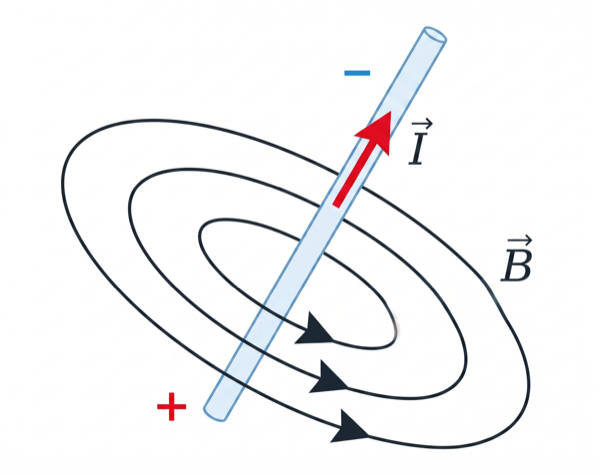
\includegraphics[width=\linewidth, keepaspectratio]{graphics/Magnetostatik_Gerader_Leiter_Magnetfeld_Wirbelfeld_B.png}
    \tcblower
    \begin{formulabox}
        \textVorFormel{Gerader Leiterabschnitt:}
        $B = \frac{\mu_0}{4\pi}\,\frac{I}{r_\perp}\,(\cos\theta_1 - \cos\theta_2)$\par
        \tcbline
        \textVorFormel{Unendlich langer gerader Leiter ($\theta_1=0^\circ, \theta_2=180^\circ$):}
        $B = \frac{\mu_0 I}{2\pi r_\perp}$
    \end{formulabox}
\end{splitbox}
\formulanote{Kreisförmige B-Feldlinien um den Leiter ($B\propto 1/r$). \ZSFkeyword{Rechte-Hand-Regel} bestimmt die Richtung. Herleitung via \ZSFref{sec:1-winkel}.}
\end{defbox}

\begin{defbox}[Lange Spule (Solenoid)]
\begin{splitbox}[0.3]
    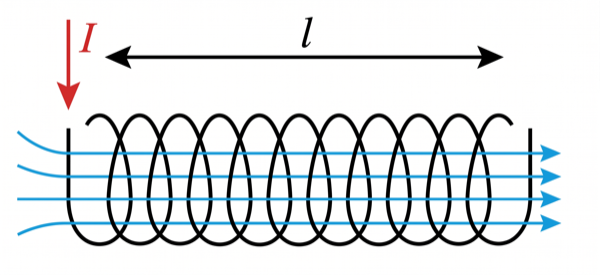
\includegraphics[width=\linewidth, keepaspectratio]{graphics/Elektrodynamik_Zylinderspule_Magnetfeld_homogen_Solenoid.png}
    \tcblower
    \begin{formulabox}
        \textVorFormel{B-Feld im Inneren:}
        $B_z = \mu_0\,\frac{N}{\ell}\,I = \mu_0\,N'\,I$
    \end{formulabox}
\end{splitbox}
\formulanote{Nahezu homogenes $\vec{B}$ im Inneren ($N$: Windungszahl, $N' = N/\ell$: Windungsdichte).}
\end{defbox}

\begin{defbox}[Ringspule (Toroid)]
\begin{splitbox}[0.3]
    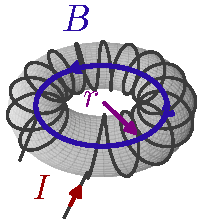
\includegraphics[width=0.72\linewidth, keepaspectratio]{graphics/Magnetfeld_Toroid_3D.pdf}
    \tcblower
    \begin{formulabox}
        \textVorFormel{B-Feld im Inneren:}
        $B = \frac{\mu_0}{2\pi}\,\frac{NI}{r}$
    \end{formulabox}
\end{splitbox}
\formulanote{$r$: Abstand vom Torus-Zentrum ($r_{\text{in}} \le r \le r_{\text{aus}}$, nicht Querschnittsradius). Geschlossene Feldlinien ($B\propto 1/r$).}
\end{defbox}

\SubsectionBar[sec:amperes-law]{Ampère}
\ZSFindex{Ampère'sches Gesetz}
\ZSFindexsee{Gesetz von Ampère}{Ampère'sches Gesetz}
\ZSFindex{Magnetischer Fluss}
\ZSFindex[Gauss-Gesetz fur Magnetfelder]{Gauss'sches Gesetz für Magnetfelder}
\ZSFindex{Durchflutung}
\begin{runintext}
Berechnung des Magnetfelds $\vec{B}$ bei \ZSFkeyword*{hoher Symmetrie} (Zylinder, Spulen, Toroid) durch das \ZSFkeyword{Linienintegral} (Zirkulation) entlang geschlossener Wege $C$.
\end{runintext}

\begin{formulabox}[Magnetischer Fluss \& Gauss'sches Gesetz]
\[ \Phi_{\mathrm{mag}} = \oint_A \vec{B}\cdot\hat{n}\,\mathrm{d}A = \oint_A B_n\,\mathrm{d}A = 0 \]
\formulanote{Zweck: Quellfreiheit des Magnetfelds (geschlossene Feldlinien, \ZSFkeyword*{keine magnetischen Monopole}). Einheit: $[\Phi_{\mathrm{mag}}] = \si{Wb} = \si{T.m^2}$.}
\end{formulabox}

\begin{formulabox}[Ampèresches Gesetz (Durchflutungsgesetz)]
\[ \oint_C \vec{B}\cdot\mathrm{d}\vec{\ell} = \mu_0\,I_C \]
\formulanote{Zweck: Zirkulation von $\vec{B}$ entlang Schleife $C$ ist proportional zur Durchflutung $I_C$ (eingeschlossener Strom; Stromdichte-Fluss \ZSFref{sec:current-drift}). \ZSFdanger{Achtung:} Orientierung von $C$ und $\hat{n}$ folgt der \ZSFkeyword{Rechte-Hand-Regel}.}
\formulasep
\[ \oint_C \vec{B}\cdot\mathrm{d}\vec{\ell} = B\,2\pi r = \mu_0\,I_C \quad \text{Zylindersymmetrie} \]
\formulanote{$C$ so wählen, dass $B$ entlang $C$ konstant und $\parallel\mathrm{d}\vec{\ell}$ ist — dann wird das Integral zu $B\cdot(\text{Weglänge})$; kein neues Gesetz.}
\end{formulabox}

\ZSFindex{Vollzylinder-Leiter}
\begin{formulabox}[Vollzylinder-Leiter (Radius $R$)]
\[ B(r) = \begin{cases} \frac{\mu_0\,I_C(r)}{2\pi r} & r \le R \quad (\text{innen}) \\[3pt] \frac{\mu_0\,I}{2\pi r} & r \ge R \quad (\text{aussen}) \end{cases} \]
\formulanote{($r$: Abstand zur Achse). Allgemein: $I_C(r) = \int_0^r J(r')\,2\pi r'\,\mathrm{d}r'$. \ZSFkeyword*{Homogen} ($J = \text{konst.}$): $I_C = I\,\frac{r^2}{R^2} \implies B_{\text{innen}} = \frac{\mu_0\,I\,r}{2\pi R^2}$ (linear steigend).}
\end{formulabox}

\begin{figbox}[Ampère-Umlauf um Spule]
    \centering
    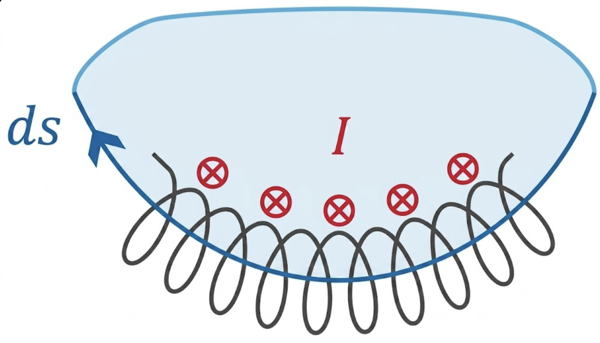
\includegraphics[width=0.86\linewidth,height=\ZSFfigMaxHeight,keepaspectratio]{graphics/Magnetismus_Solenoid_Durchflutung_Wicklungsschnitt.png}
    \ZSFfigcaption{Eingeschlossener Strom $I_C = N\cdot I$ durch Ampèresche Schleife}
\end{figbox}

\SubsectionBar[sec:magnetism-in-matter]{Magnetismus Materie}
\ZSFindex[Vakuumpermittivitat/-permeabilitat]{Vakuumpermittivität/-permeabilität}
\ZSFindex{Permeabilität}
\begin{runintext}
Ausrichtung atomarer Dipole $\vec{\mu}$ in Materie verstärkt/schwächt externes Feld $\vec{B}_{\mathrm{aus}}$ (\ZSFkeyword*{Magnetisierung} $\vec{M}$).
\end{runintext}

\begin{defbox}[Magnetisierung in Materie]
\begin{splitbox}[0.38]
    \centering
    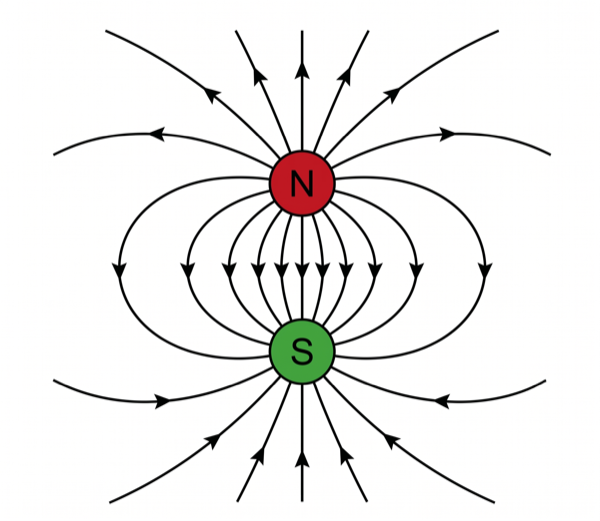
\includegraphics[width=0.88\linewidth,height=\ZSFfigMaxHeight,keepaspectratio]{graphics/Magnetismus_Dipolfeld_Feldlinienverlauf.png}
    \ZSFfigcaption{Dipolfeld (Stabmagnet)}
    \ZSFgapXS
    {\ZSFfontNote\raggedright
    \textbf{Feld- \& Dipol-Intuition:}\par
    \begin{itemize}[leftmargin=1.1em,itemsep=1pt,topsep=1pt,parsep=0pt]
      \item \textbf{Feldlinien:} Aussen N$\rightarrow$S, innen S$\rightarrow$N (geschlossen).
      \item \textbf{Ursache:} Atomare Drehimpulse $\vec{L}$ erzeugen Dipole $\vec{\mu}$.
      \item \textbf{Superposition:} Materiefeld $\mu_0\vec{M}$ überlagert äusseres Feld $\vec{B}_{\mathrm{aus}}$.
    \end{itemize}
    }
    \tcblower
    \begin{formulabox}
    \[ \vec{M} = \frac{\mathrm{d}\vec{\mu}}{\mathrm{d}V} \quad \text{Magnetisierung} \]
    \formulasep
    \[ \vec{B} = \vec{B}_{\mathrm{aus}} + \mu_0\vec{M} \]
    \[ \vec{M} = \chi_{\mathrm{mag}}\,\frac{\vec{B}_{\mathrm{aus}}}{\mu_0} \]
    \[ B = \mu_{\mathrm{rel}}\,B_{\mathrm{aus}} \]
    \[ \mu_{\mathrm{rel}} = 1 + \chi_{\mathrm{mag}} \]
    \formulasep
    \[ \vec{\mu} = \frac{q}{2m}\vec{L} \quad \text{(Atomarer Dipol)} \]
    \formulanote{Zweck: Magnetisierung $\vec{M}$, Gesamtfeld $\vec{B}$, ext. Feld $\vec{B}_{\mathrm{aus}}$. $\chi_{\mathrm{mag}}$: Suszeptibilität, $\mu_{\mathrm{rel}}$: Permeabilität, $\vec{L}$: Bahndrehimpuls.}
    \end{formulabox}
\end{splitbox}
\end{defbox}

\begin{statementbox}[Materialklassen (\ZSFkeyword[Paramagnetismus]{Para-}, \ZSFkeyword[Diamagnetismus]{Dia-}, \ZSFkeyword[Ferromagnetismus]{Ferro})]
\begin{factlist}
  \ZSFFact{Paramagnetisch ($\chi_{\mathrm{mag}}>0$)}{$\mu_{\mathrm{rel}}>1$, verstärkt Feld ($T$-abhängig). Dipole $\parallel \vec{B}_{\mathrm{aus}}$.}
  \ZSFFact{Diamagnetisch ($\chi_{\mathrm{mag}}<0$)}{$\mu_{\mathrm{rel}}<1$, schwächt Feld. Supraleiter: \mbox{$\chi_{\mathrm{mag}} = -1$}.}
  \ZSFFact{Ferromagnetisch ($\chi_{\mathrm{mag}}\gg 0$)}{$\mu_{\mathrm{rel}}\gg 1$, starke Verstärkung, Weiss-Bezirke, \ZSFkeyword*{Hysterese}.}
\end{factlist}
\ZSFgapXS
\ZSFkeyword*{Bohr-Magneton}: \\
$\mu_{\mathrm{Bohr}} = \frac{e\hbar}{2m_{\mathrm{e}}} \approx 9{,}27\times 10^{-24}\,\si{A.m^2}$ \\
Curie-Gesetz (Paramagnetismus, schwaches Feld): \\
$M \approx \frac{1}{3}\,\frac{B_{\mathrm{aus}}}{k_{\mathrm{B}}T}\,M_S$
\end{statementbox}

% ============================================================
